\chapter{Theoretical framework} % Main chapter title
\label{Chapter2TheoreticalFramework} % For referencing the chapter elsewhere, use \ref{Chapter1Introduction}
\lhead{\emph{Theoretical framework}} % This is for the header on each page - perhaps a shortened title

%----------------------------------------------------------------------------------------

Before reviewing the state of the art and compare existing solutions to this project, to better understand the contribution of this work, we will provide now an introductory overview of the theoretical concepts related to this project on \textit{stream mining} and \textit{privacy preserving} data mining mechanisms.

\section{Stream Mining}
\label{Theory::StreamMining}

Data stream mining is a relatively new field. Even though its theoretical foundation is based in well-established statistical and computational approaches, it has not been until recent years that this research area has experimented a great growth in interest.

The main problem when dealing with streaming data is the high throughput of data being analyzed, under computational resources constraints. Variable data rates is another problem that has to be addressed too. Once these problems are resolved, the same kind of data mining analysis as in the case of batch data processing are available: classification, regression or clustering tasks, as well as outlier detection and recommendation systems. We will not cover these techniques here, because they are not related to this project, by themselves. Instead, we will have a look at some different stream mining solutions, because their working principles do affect the way the project’s algorithms will be implemented.

\subsection{Stream mining approaches}
\label{Theory::StreamMining::Approaches}

Solutions provided in this field can be categorized into \textit{data-based} and \textit{task-based} ones~\citep{Gaber:MiningDataStreamsReview}, depending on their approach.

\subsubsection*{Data-based stream mining solutions}

The idea behind these solutions is to use a subset of the original dataset to perform the required analyses. Diverse techniques that have been used in this sense can further be split into two more categories:

\begin{itemize}
	\item \textbf{Sampling methods:} either by randomly picking samples of the data stream or by randomly selecting chunks (subsets) of the stream, sampling methods discard part of the incoming data, while performing the knowledge discovery processes with the sampled data. The main problem with this approach is that is hard to know when to pick a sample or which records should be stored, because there is no previous knowledge of the dataset size or its information structure.

	\item \textbf{Summarizing methods:} they use aggregated data or calculated statistical measures (that are continuously recalculated) to provide the information needed for the data mining algorithms. In this case, it is the loss of information and accuracy and the inability to control data distribution fluctuations what renders these methods not so usable as it was desired.
\end{itemize}

\begin{figure}
\centering
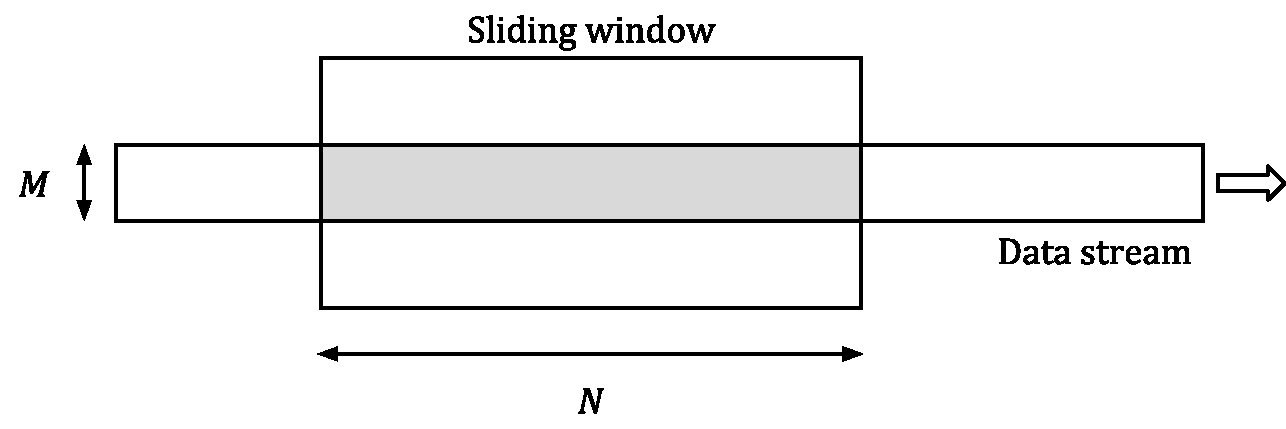
\includegraphics[width=0.9\linewidth]{figures/sliding-window.pdf}
\caption[Sliding window based stream processing.]{Processing a data stream using a \textit{sliding window} approach. In the figure, $N$ is the \textit{size} of the sliding window, in terms of the number of samples of the stream being stored, whereas $M$ is the number of \textit{attributes} of the samples in the stream.}
\label{fig:sliding-window}
\end{figure}

\subsubsection*{Task-based stream mining solutions}

The solutions that fall into this category are based not on performing data transformations, but on changing the data mining methods to enable their use on data streams.

\begin{itemize}
	\item \textbf{Approximation algorithms:} these are a kind of algorithms that are designed to solve computationally hard problems, by giving an approximate result. Instead of computing exact solutions, they just guarantee a certain error bound. The problem with these methods is, again, the high received data throughput, which they cannot cope as well. Additional tooling is therefore needed if one wishes to use them.

	\item \textbf{Sliding window method:} this method, a common pattern in many online\footnote{In computer science, an \textit{online algorithm} is one that can process its input piece-by-piece in a serial fashion, i.e., in the order that the input is fed to the algorithm, without having the entire input available from the start.} applications, maintains a \textit{sliding window} in which the most recent data is kept. As data is received from the incoming streams, this window “advances” so new observations are kept inside, as can be seen in \fref{fig:sliding-window}. The data mining analyses are then performed using the data available inside the window and summarized versions of the older records, in the form of statistical measures or aggregated data.
	This particular method is the one that the MOA package uses - thus its name: Massive \textbf{Online} Analysis. This solution scheme enables dealing with concept drift, which would not be possible if just aggregated data was used.

	\item \textbf{Algorithm output granularity:} this method is a resource-aware data analysis approach that can perform the local analysis on resource constrained devices, by adapting to resource availability and data stream rates - when resources are completely running out, the results are merged and stored.
\end{itemize}

\section{Statistical Disclosure Control}
\label{Theory:SDC}

As was already introduced in \sref{Introduction::Context::PPSM}, the purpose of Statistical Disclosure Control (SDC) is to prevent confidential information from being linked to specific individuals to whom this data belongs. We will review now some concepts related to data disclosure and SDC methods and some theoretical foundations.

\subsection{Privacy preserving algorithms} 
\label{Theory:SDC:Algorithms}

As a quick and superficial review, the algorithms\footnote{We will not cover every algorithm in detail, because some of them are not included in the scope of this project.} being used nowadays to achieve effective privacy preserving in datasets can be categorized into the following groups~\cite{Hundepool:StatisticalDisclosureControl}:

\begin{itemize}
	\item \textit{Non-perturbative data masking:} these kind of methods do not perform data values transformations. Instead, they are based in partial suppressions of records or reductions of detail of the datasets. Some examples are:
	\begin{itemize}
		\item Sampling
		\item Global recoding
		\item Top and bottom coding
		\item Local suppression
	\end{itemize}

	\item \textit{Perturbative data masking:} these methods do release the whole dataset, if required, but it is perturbed, this is, values are changed by adding them noise. This way, records are diffused and reidentifying individuals is harder. Some examples are:
	\begin{itemize}
		\item Noise masking
		\item Micro-aggregation
		\item Rank swapping
		\item Data shuffling
		\item Rounding
		\item Re-sampling
		\item PRAM
		\item MASSC
	\end{itemize}
\end{itemize}

\subsection{Disclosure \& types of variables}
\label{Theory:SDC:DisclosureTypes}

When assessing the disclosure risks of a given dataset (or data stream) we must have a look at the different kind of variables this data is composed of. We will stick to a classic~\citep{Templ:IntroSDC} categorization of such attributes into three groups, which need not be disjunctive, as follows:

\begin{itemize}
	\item \textbf{Identifiers:} variables that precisely identify individuals, e.g., social insurance numbers, person names, or addresses.
	\item \textbf{Quasi-identifiers:} a set of variables that, when considered together, can be used to identify individual units. It might be possible to, for example, identify people by combining variables such as gender, age, region and occupation.
	\item \textbf{Non-identifying variables:} these are neither \textit{identifiers} nor \textit{quasi-identifiers}.
\end{itemize}

Concerning \textit{disclosure}, it is also defined differently depending on the type of privacy breach that has occurred:

\begin{itemize}
	\item We talk about \textit{identity disclosure} when a specific individual record can be recognised in a dataset, i.e., when linkage with external available data is possible. Identity disclosure is performed using direct identifiers, rare combinations of values in quasi-identifier attributes and exact knowledge of variable values in external databases.
	\item In the case of \textit{attribute disclosure}, the intruder is able to gather sensitive information about a specific unit from the released data, where it is directly available. For example, if no perturbation is applied to the original values of the \textit{wages} variable, one could learn how much a person is earning if its identity is disclosed too.
	\item \textit{Inferential disclosure}, the most general case, occurs when an intruder is able to, with some uncertainty, predict or \textit{infer} confidential information about an individual from the statistical properties of data.
\end{itemize}

It is important to remark that a subset of critical variables might be exploited to disclose every information about a single unit in a dataset. Thus, we are bound to carefully select which variables of the dataset might be released to further users of the data, while trying to maximize its statistical utility. More concretely, it is extremely important to \textbf{not release identifiers} and to analyze quasi-identifiers closely, in order to avoid information leaks and privacy breaches.

\subsection{Disclosure Risk}
\label{Theory:SDC:DiscRisk}

Concerning the safety of the released data, \textbf{Disclosure Risk} (DR) is a common way to measure and assess the risk of re-identification of particular individuals. Re-identification happens when some sensitive and confidential data that have been released are subsequently linked to a particular individual, which results in a confidentiality breach. There are a number of different approaches in how to assess disclosure risk and whether to measure it \textit{per record} or globally, taking into account the whole dataset.

As noted in \citep{Domingo:DiscRiskAssessment}, there is not much literature on disclosure risk that can be used for a broad class of perturbative methods; disclosure risk measures tend instead to be method-specific. Therefore, empirical methods are most used to assess disclosure risk for these kind of methods.

\subsubsection{Record linkage}

Most notably, the mechanisms used to measure disclosure risk follow a \textit{record linkage} approach. This is, after an SDC method has been used to anonymize data, a record linkage procedure is applied to the original and released (masked, anonymized) datasets. This \textit{linkage} attempts to identify, for each record in the masked dataset, which is the corresponding record in the original dataset. If such correspondance is verified, the record is labeled as \textit{correctly linked}. A generic measure for disclosure risk is the percentage of correctly linked records from the total amount in the dataset.

\begin{itemize}
	\item \textbf{Distance-based record linkage:} provided that a \textit{distance} measure can be defined between the original and the masked datasets, linkage is performed as follows: for each record in the anonymized dataset, a distance to each record in the original dataset is calculated. The nearest record, in terms of this distance measurement, is assumed to be the corresponding record, thus establishing a \textit{link} between them. This linkage is then verified to assess how many of these guesses are true re-identifications.
	
	\item \textbf{Probabilistic record linkage:} in this case, the matching algoritm works a little different. For each possible pair of original and masked records, a \textit{coincidence vector} is defined. This vector holds, for each attribute, whether or not the values of the considered records are equal. An index is computed afterwards over these vectors and, using such index, the records pairs are classified as \textit{linked} or \textit{not linked}. Again, this linkage is verified to assess the number of true re-identifications.
\end{itemize}

\subsection{Information Loss}
\label{Theory:SDC:InfoLoss}

Another key measurement concerning data protection is \textbf{Information Loss} (IL) or \textit{data utility}, which could be defined as the amount of useful statistical information that is lost along the data masking process. A good SDC method should try to minimize IL, in order to provide optimally useful data to the legitimate users of such data, while also keeping a low disclosure risk. It is important to note that these two properties are inversely proportional: the lower disclosure risk is, the higher information loss will occur. This trade off between these two parameters is often a difficult and challenging task and should be taken into very careful consideration, depending on the release policies that apply, the kind of data being released and the sensitivity of the information contained in such data. This evaluation should be performed not only from a purely quantitave and numerical point of view, but from an ethical and privacy concerned one too.

As well as with disclosure risk, a number of methods and approaches are taken to assess information loss when releasing privacy protected datasets, ranging from unbounded~\citep{Domingo:SDCMethodsInfoLoss} to probabilistic (bound to the $[0,1]$ interval) measurements~\citep{Mateo:ProbInfLossMeasures}.

\subsubsection*{Unbounded Information Loss}

An example framework to assess IL was given in \citep{Domingo:SDCMethodsInfoLoss}, which evaluates some key statistical properties of the released data. More concretely, it computes three \textit{discrepancy} measurements for a series of pairs of matrices (correlation, covariance, etc. of the original and masked datasets), namely the \textit{mean square error}, the \textit{mean absolute error} and the \textit{mean variation}.

\subsubsection*{Probabilistic Information Loss}

The aim of measuring IL in a probabilistic manner is to bound this measurement to the $[0,1]$ range, thus allowing its comparison with DR, which is also generally expressed within this range. This way, a \textit{score} could be calculated from both normalized measures for an SDC method, easing parameters selection to data protectors, for example.

\subsection{Privacy guarantees}
\label{Theory:SDC:Guarantees}

Many different methods have been developed to help prevent information disclosure when data mining datasets or results are released. These algorithms pursue the generation of results or data that have particular properties concerning privacy preservation. Some of the desirable properties of privacy-protected data are described in the following sections, but no formal definition is provided for some of them (please refer to the original papers and publications to understand them better).

\subsubsection{\textit{k}-Anonymity}

First described in 2002, by Latanya Sweeney, a release of data is said to have the \textit{$k$-anonymity} property if the information for each person contained in the release cannot be distinguished from at least $k-1$ individuals whose information also appears in the release~\citep{Sweeney:kAnonymity}. A more formal definition uses the previously reviewed concept of \textit{quasi-identifiers} (see~\sref{Theory:SDC:DisclosureTypes}).

\begin{definition}~($k$-Anonymity)
A dataset is said to satisfy $k$-anonymity for an integer $k > 1$ if, for each combination of values of quasi-identifiers, at least $k$ records exist in the dataset sharing that combination.~\citep{Domingo:EnhancingDiffPrivMicroaggregation}
\end{definition}

An intruder trying to use a $k$-anonymous dataset to do, for example, record linkage against an external source of information will find that at least $k$ records in the dataset match any value of the quasi-identifiers that he or she is trying to use to perform the linkage. Thus, re-identification is limited to \textit{groups}, this is, no individual records can be linked, just groups of size at least $k$.

\subsubsection{\textit{l}-Diversity}

The evolution of the concept of $k$-anonymity is \textit{$l$-diversity} and adds further privacy preservation by adding intra-group diversity, so to avoid the flaws of the $k$-anonymity privacy model~\citep{Machanavajjhala:lDiversity}.

\subsubsection{\textit{t}-Closeness}

Further on, the \textit{$t$-closeness} property definition adds attribute-based privacy enforcement to the $l$-diversity model: to better preserve privacy, all values (all observations) from a particular attribute must not be too much different - instead, they should be close up to a certain threshold~\citep{Ninghui:tCloseness}. This is needed to preserve the privacy of those records that are more easily identifiable because their attribute values are more distinguishable.

\subsubsection{Differential Privacy}

Described in~\citet{Dwork:DifferentialPrivacy}, \textit{differential privacy} is a condition \textit{on the release mechanism} (not the dataset) that guarantees a strong privacy preservation level for some particular data uses contexts. Differential privacy is introduced in an \textit{interactive} setting, i.e., in a query-response data retrieval environment, and offers probabilistic guarantees that the contribution of any single individual to thenquery response is limited.

\begin{definition}~($\varepsilon$-Differential privacy)
A randomized mechanism\footnote{By \textit{mechanism}, we refer to any kind of function or system used to query for data.} $\mathcal{M}$ gives $\varepsilon$-differential privacy if, for all datasets $X_1$, $X_2$ such that one can be obtained from the other by modifying a \textit{single} record, and all $S \subset Range(\mathcal{M})$, it holds
\begin{equation}
P(\mathcal{M}(X_1) \in S) \leq \mathrm{exp}(\varepsilon) \times P(\mathcal{M}(X_2) \in S)
\end{equation}
\end{definition}

This definition, cited from~\citet{Domingo:EnhancingDiffPrivMicroaggregation}, easier to understand than the original one given in~\citet{Dwork:DifferentialPrivacy}, states that, given an $\varepsilon$-differential privacy mechanism $\mathcal{M}$ and any possible output $r$, the presence or abscence of a participant (in terms of the dataset, a \textit{row}) will cause at most a multiplicative $e^\varepsilon$ change in the probability of the mechanism to output a response $r$.
\section{SDC methods}
\label{Theory:SDCMethods}

We will describe now some of the most common methods and mechanisms used in SDC applications to anonymize data or provide privacy preserving data releases.

\subsection*{Notation}

We assume the following notation for the subsequent method descriptions:

\begin{itemize}
	\item
	The original dataset is the matrix $X$, with $n$ rows (samples) and $m$ attributes or variables. Therefore, the $x_{ij}$ element of the dataset denotes the value that the $j$-th attribute takes in the $i$-th row for any $1 \leq i \leq n$ and $1 \leq j \leq m$.
	
	\item
	The anonymized (protected) dataset is named $X'$.
\end{itemize}

\subsection{Noise Addition}
\label{Theory:SDCMethods:NoiseAddition}

Noise addition or \textit{additive noise masking} is a fairly simple method that is based on the addition of gaussian noise to data, thus randomly distorting its values and difficulting re-identification of individuals. The main additive noise algorithms in the literature are~\citep[p. 54]{Hundepool:StatisticalDisclosureControl}:

\begin{itemize}
	\item
	Uncorrelated noise addition.
	\item
	Correlated noise addition.
	\item
	Noise addition and linear transformation.
	\item
	Noise addition and non-linear transformation.
\end{itemize}

We will only cover the first couple of methods, because of the inherent difficulty of the latter, both in its theoretical basis and its practical implementation, which renders them not suitable for the needs of this project.

\subsubsection{Uncorrelated noise addition}

Masking by additive noise the $j$-th variable of an original dataset $X$ yields an anonymized dataset $X'$ such that

\begin{equation}
x_{ij}' = x_{ij} + \epsilon\ \ \ \text{for}\ 1 \leq i \leq n
\end{equation}

where $\epsilon$ is drawn from a random variable $\varepsilon_j \sim N(0,\sigma_{\varepsilon_j}^2)$. The general assumption is that the variances of each $\varepsilon_j$ are proportional to those of the original variables, this is, if $\textrm{Var}(X_j) = \sigma_j^2$ is the variance of the $j$-th attibute of the dataset $X$, then $\sigma_{\varepsilon_j}^2 := \alpha\sigma_j^2$.

While this method preserves means and covariances, it is, unfortunately, not able to preserve variances nor correlation coefficients.

\subsubsection{Correlated noise addition}

This method is aimed to also preserve correlation coefficients, with respect to \textit{uncorrelated} noise addition. The main difference with the previous mechanism is that the covariance matrix of the errors is now proportional to the covariance matrix of the data: $\varepsilon \sim N(0,\Sigma_\varepsilon)$, where $\Sigma_\varepsilon = \alpha\Sigma$.

Masking by correlated noise addition provides data with higher analytical utility than masking using uncorrelated noise, as long as $\alpha$ is revealed to the data user. However, the low level of protection yielded by this method and the previous one render them as not very useful for truly important SDC applications.

\subsection{Microaggregation}
\label{Theory:SDCMethods:Microaggregation}

Originally described for continuous (numerical) data, microaggregation is a family of SDC methods that, in the most general form, consist of making homogeneous groups of $k$ or more individuals (rows) from within the $X$ dataset to later replace their values with aggregated ones, this is, averages, computed on the groups themselves. These grouped and aggregated records conform the resulting $X'$ release dataset.

Two main approaches are taken when considering microaggregation techniques: \textit{univariate} and \textit{multivariate} microaggregation. The difference remains in the number of variables used to perform the \textit{clustering} phase of the method: a single variable and multiple attributes, correspondingly. As can be assessed in the literature, the univariate approach causes either a very high information loss or a very high disclosure risk, thus not being appropriate for normal SDC uses~\citep[p. 63]{Hundepool:StatisticalDisclosureControl}. On the other hand, multivariate microaggregation, proposed by~\citet{Domingo:PracticalMicroaggregation}, is considered an excellent protection method and, as such, we will focus on this approach.

It is important to note that this family of techniques are directly related to $k$-anonymity, as proved in~\citet{Domingo:KAnonMicroagg}.

\subsubsection{Partition}

The first and most computational complex task to do in a microaggregation method is to partition the dataset into $g$ groups of size at least $k > 1$, which is, indeed, a \textit{clustering} task. This proves to be quite difficult, but an optimal solution approximation with respect to information loss was already given in~\citep{Domingo:KAnonMicroagg} and further refined in~\citet{Domingo:MuAproxPolyTimeMicroagg}.

The aim of these partition methods is to find the optimal $k$-partition that maximizes within-group homogeneity. Following~\citet{Domingo:PracticalMicroaggregation}, a practical information loss measure for microaggregation, relatively common in the clustering literature, is the ratio of within-group homogeneity over the total sum of squares (the sum of \textit{within} and \textit{between} group homogeneity)

\begin{equation}\label{eq:clustering-info-loss}
L = \frac{SSE}{SST}
\end{equation}

The within-group homogeneity ($SSE$) is defined as

\begin{equation}
SSE = \sum_{i=1}^{g} \sum_{j=1}^{n_i} (x_{ij} - \mathbf{\bar{x}_i})^2
\end{equation}

where $g$ denotes the total number of groups of $n_i$ elements each and $\mathbf{\bar{x}_i}$ denotes the $i$-th group centroid. The between-groups sum of squares, $SSA$, is

\begin{equation}
SSA = \sum_{i=1}^{g} n_i (\mathbf{\bar{x}_i} - \mathbf{\bar{x}})^2
\end{equation}

where $\mathbf{\bar{x}}$ is the average vector over the whole dataset. The total sum of squares is, then, $SST = SSE + SSA$.

Because microaggregation replaces values in a group by the group centroid, if we recall~\eref{eq:clustering-info-loss}, it follows that the higher the within-group homogeneity, the lower the information loss is. Both the MDAV~\citep{Domingo:KAnonMicroagg} (Maximum Distance to Average Vector) and $\mu$-Approx~\citep{Domingo:MuAproxPolyTimeMicroagg} algorithms are built to partition the dataset into groups, while minimizing information loss, exploiting the previous theoretical result.

\subsubsection{Aggregation}

The aggregation step is the simplest of the ones that take place in a microaggregation setting: for each group $g$ of at least $k$ records and for each attribute $1 \leq j \leq m$, an \textit{aggregate} $\gamma$ is computed among the values of the $j$-th variable for the records in the group. This aggregate is then imputed to each record for its $j$-th attribute.

Concerning the types of variables that are aggregated~\citep{Domingo:KAnonMicroagg}:

\begin{itemize}
	\item
	\textbf{Continuous attributes:} the aggregated value correponds with the arithmetical mean of the selected values.
	\item
	\textbf{Categorical attributes:} the aggregated value should either be the median or the mode of the selected values.
\end{itemize}

\subsection{Rank Swapping}
\label{Theory:SDCMethods:RankSwapping}

%TODO
\todo{rank swapping}

\subsection{Laplacian Mechanism}
\label{Theory:SDCMethods:LaplacianMechanism}

%TODO
\todo{Laplacian}
